\chapter{Teoria do campo ligante e cor}\label{ch:b2:ligand-field}

O rubi é vermelho e a esmeralda é verde, e no entanto ambos devem sua cor ao
mesmo íon, \ce{Cr^3+}, alguns dos quais substituem o alumínio no coríndon,
\ce{Al2O3}, ou no berilo. Os cristais de sulfato de cobre são de um azul
intenso, mas o pó que resta depois de aquecê-los é branco. Em cada caso, a cor
vem de elétrons que saltam entre orbitais d cujas energias os átomos vizinhos
afastaram --- de um valor que depende de quais átomos cercam o íon e de como o
cercam. Este capítulo calcula esse desdobramento, primeiro com cargas
pontuais, depois com \omterm{def:b2:diatomic-mos:lcao}{orbitais moleculares}; ele explica as cores, o magnetismo
e a \omterm{def:b2:coordination-complexes:electron-count}{regra dos 18 elétrons} do capítulo anterior.

\begin{recall}
\Cref{ch:b2:coordination-complexes}: configurações $d^n$, geometrias,
contagens de elétrons. \Cref{ch:b2:atomic-orbitals}: as formas dos cinco
orbitais d. \Cref{ch:b2:fragment-orbitals}: os \omterm{def:b2:fragment-orbitals:fragment}{orbitais de fragmento}. O volume
do 1.º ano: absorbância, cores complementares, elétrons desemparelhados, regra
de Hund.
\end{recall}

\begin{omfigure}
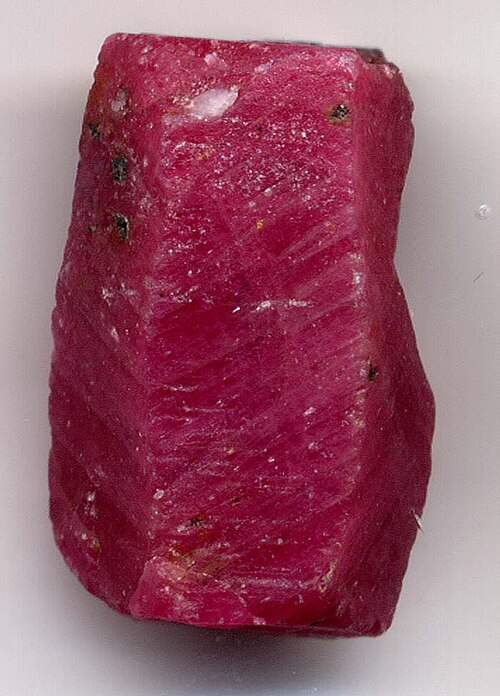
\includegraphics[height=3.6cm]{images/book3/ruby.jpg}\hspace{0.6cm}%
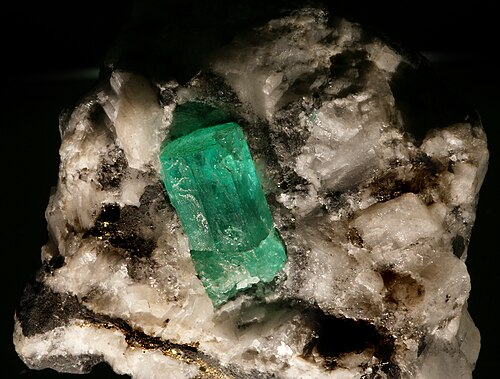
\includegraphics[height=3.6cm]{images/book3/emerald.jpg}\hspace{0.6cm}%
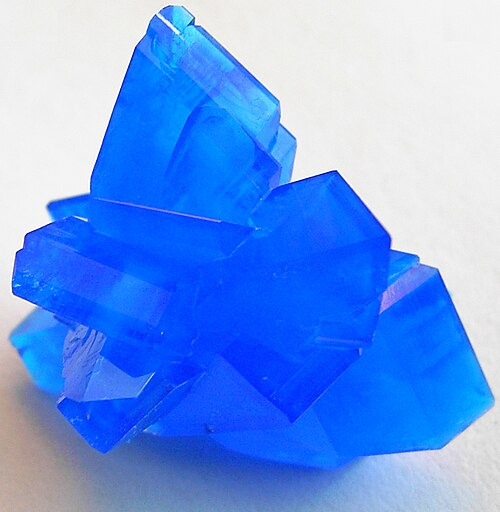
\includegraphics[height=3.6cm]{images/book3/copper-sulfate.jpg}

{\small Um cristal de rubi (domínio público); uma esmeralda em sua rocha
(Didier Descouens, CC BY-SA 3.0); cristais de sulfato de cobre(II)
penta-hidratado (Stephanb, CC BY-SA 3.0). Wikimedia Commons. O cromo(III)
colore os dois primeiros; o aquacomplexo de cobre(II), o terceiro.}
\end{omfigure}

\section{O modelo do campo cristalino}

\begin{definition}[Campo cristalino]\label{def:b2:ligand-field:crystal-field}
O \emph{modelo do campo cristalino}\index{modelo do campo cristalino} trata os ligantes de um
complexo como cargas pontuais negativas (ou as extremidades negativas de
dipolos) em torno do íon metálico, e calcula como eles mudam as energias de
seus orbitais d. Em um campo octaédrico, os orbitais d se desdobram em dois
conjuntos separados pelo \emph{desdobramento do campo
cristalino}\index{desdobramento do campo cristalino} $\Delta_o$.
\end{definition}

Coloque os seis ligantes sobre os eixos. Os orbitais $\mathrm d_{z^2}$ e
$\mathrm d_{x^2-y^2}$ apontam seus lobos diretamente para os ligantes: um elétron
neles é mais repelido, e eles sobem. Os orbitais $\mathrm d_{xy}$, $\mathrm d_{xz}$,
$\mathrm d_{yz}$ apontam entre os ligantes e sobem menos. O primeiro par se
chama $e_g$; o segundo conjunto, de três, $t_{2g}$ (nomes vindos da teoria de
grupos, no volume do 3.º ano).

\begin{omfigure}
\begin{tikzpicture}[font=\small]
  \begin{scope}
    \pic at (0,0) {omdx2y2};
    \foreach \p in {(1.25,0),(-1.25,0),(0,1.25),(0,-1.25)} \node[circle, fill=black!70, inner sep=2.2pt] at \p {};
    \node at (0,-1.75) {$\mathrm d_{x^2-y^2}$: lobos voltados para os ligantes};
  \end{scope}
  \begin{scope}[xshift=5.5cm]
    \pic at (0,0) {omdxy};
    \foreach \p in {(1.25,0),(-1.25,0),(0,1.25),(0,-1.25)} \node[circle, fill=black!70, inner sep=2.2pt] at \p {};
    \node at (0,-1.75) {$\mathrm d_{xy}$: lobos entre eles};
  \end{scope}
\end{tikzpicture}

{\small Dois orbitais d entre os quatro ligantes do plano $xy$ de um octaedro
(pontos pretos). Os lobos de $\mathrm d_{x^2-y^2}$ apontam para os ligantes; os de
$\mathrm d_{xy}$, entre eles.}
\end{omfigure}

\begin{theorem}[Baricentro]\label{thm:b2:ligand-field:barycentre}
Em um campo octaédrico, medidas a partir da energia média dos orbitais d, o par
$e_g$ fica em $+0.6\Delta_o$ e o conjunto $t_{2g}$ em $-0.4\Delta_o$.
\end{theorem}

\begin{proof}
O campo eleva a média das cinco energias d, mas não a altera ao desdobrá-las
(a regra do baricentro, admitida: a soma dos deslocamentos de um conjunto
completo de orbitais é fixada pela carga total, e não por seu arranjo). Com
$e_g$ em $x$ e
$t_{2g}$ em $x - \Delta_o$, a condição $2x + 3(x - \Delta_o) = 0$ dá $x = 0.6\Delta_o$.
\end{proof}

\section{Spin alto e spin baixo}

\begin{definition}[Estados de spin]\label{def:b2:ligand-field:spin}
A \emph{energia de emparelhamento}\index{energia de emparelhamento} $P$ é a energia
necessária para colocar um segundo elétron em um orbital ocupado em vez de em
um orbital vazio de mesma energia. Um complexo é de \emph{spin alto}\index{spin alto}
quando seus elétrons ocupam os orbitais $e_g$ antes de se emparelharem em
$t_{2g}$, e de \emph{spin baixo}\index{spin baixo} quando se emparelham primeiro em
$t_{2g}$.
\end{definition}

\begin{proposition}[Escolha do estado de spin]\label{prop:b2:ligand-field:spin-state}
Para os íons octaédricos $d^4$ a $d^7$, o complexo é de \omterm{def:b2:ligand-field:spin}{spin baixo} se $\Delta_o > P$ e de
\omterm{def:b2:ligand-field:spin}{spin alto} se $\Delta_o < P$. Para $d^1$--$d^3$ e $d^8$--$d^{10}$, existe uma única configuração.
\end{proposition}

\begin{proof}
A partir de $d^3$ ($t_{2g}^3$), o quarto elétron entra em $e_g$ (custo $\Delta_o$ acima de
$t_{2g}$) ou se emparelha em $t_{2g}$ (custo $P$). Vence o mais barato; a mesma
comparação vale para cada elétron até $d^7$. Para $d^1$--$d^3$, há lugar em
$t_{2g}$ sem emparelhamento; para $d^8$--$d^{10}$, $t_{2g}$ está cheio e $e_g$ precisa
ser usado de qualquer modo.
\end{proof}

\begin{definition}[Energia de estabilização do campo cristalino]\label{def:b2:ligand-field:cfse}
A \emph{energia de estabilização do campo cristalino}\index{energia de estabilizacao do campo cristalino@energia de estabilização do campo cristalino}
(EECC) de uma configuração $t_{2g}^ae_g^b$ é $(-0.4a + 0.6b)\Delta_o$, a energia
dos elétrons d em relação ao baricentro (com as \omterm{def:b2:ligand-field:spin}{energias de emparelhamento}
contadas à parte).
\end{definition}

\begin{proposition}[EECC ao longo da série]\label{prop:b2:ligand-field:cfse}
Em \omterm{def:b2:ligand-field:spin}{spin alto}, a EECC vale $0$, $-0.4$, $-0.8$, $-1.2$, $-0.6$, $0$, $-0.4$, $-0.8$, $-1.2$,
$-0.6$, $0$ (em $\Delta_o$) de $d^0$ a $d^{10}$: ela se anula para $d^0$, $d^5$,
$d^{10}$. Em \omterm{def:b2:ligand-field:spin}{spin baixo}, ela chega a $-2.4\Delta_o$ para $d^6$.
\end{proposition}

\begin{proof}
Preencha as configurações e aplique a definição; os valores são os da figura,
calculados.
\end{proof}

\begin{omfigure}
\begin{tikzpicture}
\begin{axis}[width=0.55\linewidth, height=5cm, xmin=-0.5, xmax=10.5, ymin=-2.6, ymax=0.3,
  axis x line=bottom, axis y line=left, xlabel={$d^n$}, ylabel={EECC ($\Delta_o$)},
  xtick={0,1,2,3,4,5,6,7,8,9,10}, tick label style={font=\small}, label style={font=\small}]
\addplot[omThm, thick, mark=*, mark size=1.3pt] table[x=n, y=high] {figdata/out/bachelor-2-ligand-field-a.dat};
\addplot[omDef, thick, dashed, mark=square*, mark size=1.3pt] table[x=n, y=low] {figdata/out/bachelor-2-ligand-field-a.dat};
\node[font=\scriptsize, omThm, anchor=west] at (axis cs:5.4,0.0) {spin alto};
\node[font=\scriptsize, omDef, anchor=west] at (axis cs:6.6,-2.2) {spin baixo};
\end{axis}
\end{tikzpicture}\hfill
\begin{tikzpicture}[font=\small]
  \pic (t) at (0,0) {omlevel={ud}{0.5}}; \pic at (0.6,0) {omlevel={u}{0.5}}; \pic at (1.2,0) {omlevel={u}{0.5}};
  \pic at (0.3,1.6) {omlevel={u}{0.5}}; \pic at (0.9,1.6) {omlevel={u}{0.5}};
  \node at (0.6,-0.8) {$d^6$ de spin alto};
  \node[font=\scriptsize, anchor=east] at (-0.35,0) {$t_{2g}$}; \node[font=\scriptsize, anchor=east] at (-0.05,1.6) {$e_g$};
  \pic at (3,0) {omlevel={ud}{0.5}}; \pic at (3.6,0) {omlevel={ud}{0.5}}; \pic at (4.2,0) {omlevel={ud}{0.5}};
  \pic at (3.3,2.4) {omlevel={empty}{0.5}}; \pic at (3.9,2.4) {omlevel={empty}{0.5}};
  \node at (3.6,-0.8) {$d^6$ de spin baixo};
  \draw[<->, omProp] (4.7,0) -- (4.7,2.4) node[midway, right, font=\scriptsize] {$\Delta_o$};
  \draw[<->, omProp] (1.7,0) -- (1.7,1.6) node[midway, right, font=\scriptsize] {$\Delta_o$};
\end{tikzpicture}

{\small À esquerda: \omterm{def:b2:ligand-field:cfse}{energia de estabilização do campo cristalino} ao longo da
série d (calculada), \omterm{def:b2:ligand-field:spin}{spin alto} (contínua) e \omterm{def:b2:ligand-field:spin}{spin baixo} (tracejada). À direita:
as duas configurações de um íon $d^6$: quatro elétrons desemparelhados quando
$\Delta_o < P$ (como \ce{[Fe(H2O)6]^2+}), nenhum quando $\Delta_o >
P$ (como \ce{[Fe(CN)6]^4-}).}
\end{omfigure}

\begin{method}[Estado de spin, EECC e elétrons desemparelhados]\label{met:b2:ligand-field:spin-state}
\begin{enumerate}
  \item Encontre $n$ a partir do estado de oxidação ($n = g - m$).
  \item Para $d^4$--$d^7$, compare $\Delta_o$ e $P$ (ou situe o ligante na \omterm{def:b2:ligand-field:spectrochemical}{série
        espectroquímica}): campo forte, \omterm{def:b2:ligand-field:spin}{spin baixo}; campo fraco, \omterm{def:b2:ligand-field:spin}{spin alto}.
  \item Preencha $t_{2g}$ e $e_g$ em conformidade; EECC $= (-0.4a + 0.6b)\Delta_o$.
  \item Conte os elétrons desemparelhados; qualquer elétron desemparelhado
        torna o complexo \omterm{def:b2:diatomic-mos:magnetism}{paramagnético}.
\end{enumerate}
\end{method}

\section{Outras geometrias}

\begin{proposition}[Campos tetraédrico e quadrado plano]\label{prop:b2:ligand-field:tetrahedral}
Em um campo tetraédrico, a ordem se inverte: dois orbitais ($e$) abaixo de três ($t_2$),
com um desdobramento $\Delta_t \approx \frac49\Delta_o$ para o mesmo metal e os mesmos
ligantes; os complexos tetraédricos são de \omterm{def:b2:ligand-field:spin}{spin alto}. Em um campo quadrado
plano, o orbital $\mathrm d_{x^2-y^2}$ fica muito acima dos outros: um íon $d^8$
preenche os quatro orbitais inferiores e o deixa vazio.
\end{proposition}

\admitted

O fator $4/9$ vem da geometria das cargas pontuais; com apenas quatro
ligantes, nenhum apontando ao longo dos eixos, o desdobramento é pequeno demais
para vencer a \omterm{def:b2:ligand-field:spin}{energia de emparelhamento}. Retirar os dois ligantes do eixo $z$
de um octaedro abaixa os orbitais com componente em $z$ e não eleva nenhum:
isso explica os complexos $d^8$ quadrados planos do capítulo anterior, cujos
oito elétrons encontram todos lugar abaixo do $\mathrm d_{x^2-y^2}$ vazio.

\begin{omfigure}
\begin{tikzpicture}[font=\scriptsize]
  % octahedral
  \pic at (-0.3,0) {omlevel={empty}{0.45}}; \pic at (0.25,0) {omlevel={empty}{0.45}}; \pic at (0.8,0) {omlevel={empty}{0.45}};
  \pic at (0,1.8) {omlevel={empty}{0.45}}; \pic at (0.55,1.8) {omlevel={empty}{0.45}};
  \node[anchor=west] at (1.1,0) {$t_{2g}$}; \node[anchor=west] at (0.85,1.8) {$e_g$};
  \node[font=\small] at (0.25,-0.7) {octaédrico};
  % tetrahedral
  \begin{scope}[xshift=3.5cm]
    \pic at (0,0.6) {omlevel={empty}{0.45}}; \pic at (0.55,0.6) {omlevel={empty}{0.45}};
    \pic at (-0.3,1.4) {omlevel={empty}{0.45}}; \pic at (0.25,1.4) {omlevel={empty}{0.45}}; \pic at (0.8,1.4) {omlevel={empty}{0.45}};
    \node[anchor=west] at (0.85,0.6) {$e$}; \node[anchor=west] at (1.1,1.4) {$t_2$};
    \node[font=\small] at (0.25,-0.7) {tetraédrico};
  \end{scope}
  % square planar
  \begin{scope}[xshift=7cm]
    \pic at (0,-0.2) {omlevel={empty}{0.45}}; \pic at (0.55,-0.2) {omlevel={empty}{0.45}};
    \pic at (0.25,0.3) {omlevel={empty}{0.45}};
    \pic at (0.25,0.9) {omlevel={empty}{0.45}};
    \pic at (0.25,2.6) {omlevel={empty}{0.45}};
    \node[anchor=west] at (0.85,-0.2) {$\mathrm d_{xz}, \mathrm d_{yz}$};
    \node[anchor=west] at (0.55,0.3) {$\mathrm d_{z^2}$};
    \node[anchor=west] at (0.55,0.9) {$\mathrm d_{xy}$};
    \node[anchor=west] at (0.55,2.6) {$\mathrm d_{x^2-y^2}$};
    \node[font=\small] at (0.25,-0.7) {quadrado plano};
  \end{scope}
\end{tikzpicture}

{\small Desdobramento dos orbitais d em três geometrias, esquemático (não na
mesma escala): octaédrica, tetraédrica (invertido e menor), quadrada plana (um
orbital muito acima dos outros).}
\end{omfigure}

\section{A cor e a série espectroquímica}

\begin{definition}[Transição d--d]\label{def:b2:ligand-field:d-d}
Uma \emph{transição d--d}\index{transicao d--d@transição d--d} é a promoção de um elétron de um
nível d inferior a um nível d superior de um complexo por absorção de luz;
para um íon $d^1$, de $t_{2g}$ a $e_g$, com a energia $\Delta_o$.
\end{definition}

\begin{proposition}[O desdobramento a partir da cor]\label{prop:b2:ligand-field:colour}
Se um complexo absorve mais fortemente no comprimento de onda $\lambda_{\max}$ por
uma \omterm{def:b2:ligand-field:d-d}{transição d--d} de energia $\Delta_o$, então $\Delta_o = N_Ahc/\lambda_{\max}$ por
mol, ou $\tilde\nu = 1/\lambda_{\max}$ em número de onda; a cor vista é a
complementar da cor absorvida.
\end{proposition}

\begin{proof}
Um fóton de comprimento de onda $\lambda$ carrega $hc/\lambda$; um mol de fótons, $N_Ahc/\lambda$. A
luz branca menos a banda absorvida aparece na cor complementar.
\end{proof}

\begin{method}[De uma banda de absorção a uma cor]\label{met:b2:ligand-field:colour}
\begin{enumerate}
  \item Converta $\lambda_{\max}$ em $\tilde\nu = 1/\lambda_{\max}$ (\unit{cm^{-1}}) e em
        $N_Ahc/\lambda_{\max}$ (\unit{kJ/mol}): $\qty{500}{nm} \leftrightarrow \qty{20000}{cm^{-1}}
        \leftrightarrow \qty{239}{kJ/mol}$.
  \item Encontre a cor absorvida (violeta 400--430, azul 430--490, verde 490--560,
        amarelo 560--590, laranja 590--620, vermelho 620--700 nm, aproximadamente).
  \item A cor vista é a oposta no círculo cromático.
\end{enumerate}
\end{method}

\begin{omfigure}
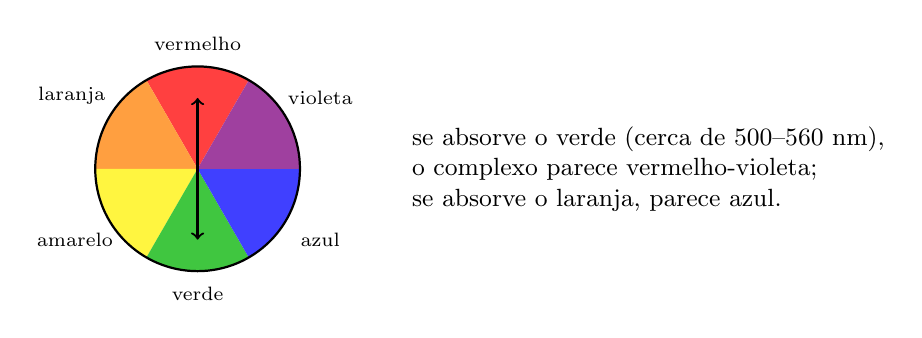
\begin{tikzpicture}[font=\scriptsize]
  \foreach \a/\c/\n in {90/red/vermelho, 150/orange/laranja, 210/yellow/amarelo, 270/green!70!black/verde, 330/blue/azul, 30/violet/violeta} {
    \fill[\c!75] (0,0) -- (\a-30:1.3) arc[start angle=\a-30, end angle=\a+30, radius=1.3] -- cycle;
    \node[anchor=\a+180] at (\a:1.38) {\n};
  }
  \draw[thick] (0,0) circle (1.3);
  \draw[<->, thick] (90:0.9) -- (270:0.9);
  \node[anchor=west, font=\small, align=left] at (2.6,0) {se absorve o verde (cerca de 500--560 nm),\\ o complexo parece vermelho-violeta;\\ se absorve o laranja, parece azul.};
\end{tikzpicture}

{\small Um círculo cromático: a cor vista é aproximadamente a complementar,
diametralmente oposta, da banda absorvida.}
\end{omfigure}

\begin{definition}[Série espectroquímica]\label{def:b2:ligand-field:spectrochemical}
A \emph{série espectroquímica}\index{serie espectroquimica@série espectroquímica} ordena os ligantes
pelo desdobramento que produzem para um dado íon metálico:
\[
  \ce{I-} < \ce{Br-} < \ce{Cl-} < \ce{F-} < \ce{OH-} < \ce{H2O} < \ce{NH3} < \text{en} <
  \ce{NO2-} < \ce{CN-} < \ce{CO} .
\]
Para um dado ligante, $\Delta_o$ também cresce com a carga do íon metálico e
descendo um grupo (os complexos 4d e 5d, maiores que os 3d, são quase sempre de
\omterm{def:b2:ligand-field:spin}{spin baixo}).
\end{definition}

Os haletos estão na extremidade fraca, e \ce{CN-} e \ce{CO} na extremidade
forte, o que o \omterm{def:b2:ligand-field:crystal-field}{modelo do campo cristalino} não consegue explicar: ele colocaria
o \ce{F-}, carregado, acima do \ce{CO}, neutro. A explicação exige orbitais.

\section{O campo ligante}

\begin{definition}[Teoria do campo ligante]\label{def:b2:ligand-field:ligand-field}
A \emph{teoria do campo ligante}\index{teoria do campo ligante} descreve um complexo com
\omterm{def:b2:diatomic-mos:lcao}{orbitais moleculares} construídos a partir dos orbitais de valência do metal
(seus nove orbitais $n$d, $(n+1)$s e $(n+1)$p) e dos orbitais doadores dos
ligantes.
\end{definition}

\begin{proposition}[Ligação $\sigma$ em um complexo octaédrico]\label{prop:b2:ligand-field:mo-octahedral}
Com seis ligantes, cada um cedendo um orbital doador $\sigma$, formam-se seis
\omterm{def:b2:diatomic-mos:lcao}{orbitais moleculares} ligantes a partir do s, dos três p e dos dois orbitais d
$e_g$ do metal; os três orbitais $t_{2g}$, que apontam entre os ligantes,
permanecem não ligantes; acima deles ficam os \omterm{def:b2:diatomic-mos:bonding}{orbitais antiligantes} $e_g^*$. Os
elétrons dos ligantes preenchem os seis \omterm{def:b2:diatomic-mos:bonding}{orbitais ligantes}; os elétrons d do
metal vão para $t_{2g}$ e $e_g^*$, separados por $\Delta_o$. Os \omterm{def:b2:diatomic-mos:bonding}{orbitais
ligantes} e não ligantes podem conter $12 + 6 = 18$ elétrons.
\end{proposition}

\begin{proof}[Raciocínio]
Pelo método dos fragmentos do \cref{ch:b2:fragment-orbitals}, cada orbital do
metal interage com a combinação de orbitais dos ligantes de mesma simetria: o
s com a totalmente simétrica, cada p com um par de ligantes opostos, $\mathrm d_{z^2}$ e $\mathrm
d_{x^2-y^2}$ com as combinações voltadas para seus lobos; nenhuma combinação
$\sigma$ corresponde aos orbitais $t_{2g}$ (sua sobreposição com qualquer doador
$\sigma$ que aponte ao longo de um eixo é nula por simetria). Os nomes das
combinações vêm da teoria de grupos, admitida. Preencher todos os \omterm{def:b2:diatomic-mos:bonding}{orbitais
ligantes} e não ligantes, e nenhum dos antiligantes, exige
18 elétrons --- a \omterm{def:b2:coordination-complexes:electron-count}{regra dos 18 elétrons}.
\end{proof}

\begin{omfigure}
\begin{tikzpicture}[font=\scriptsize]
  % metal
  \pic (m4p1) at (-0.45,2.6) {omlevel={empty}{0.4}}; \pic (m4p2) at (0,2.6) {omlevel={empty}{0.4}}; \pic (m4p3) at (0.45,2.6) {omlevel={empty}{0.4}};
  \node[anchor=east] at (-0.7,2.6) {$(n{+}1)$p};
  \pic (m4s) at (0,1.8) {omlevel={empty}{0.6}}; \node[anchor=east] at (-0.35,1.8) {$(n{+}1)$s};
  \foreach \x in {-0.9,-0.45,0,0.45,0.9} \pic at (\x,0.6) {omlevel={empty}{0.4}};
  \coordinate (m3d) at (1.1,0.6); \node[anchor=east] at (-1.15,0.6) {$n$d};
  \node[font=\small] at (0,-2.9) {metal};
  % ligands
  \foreach \x in {6.2,6.72,7.24,7.76,8.28,8.8} \pic at (\x,-0.9) {omlevel={ud}{0.36}};
  \coordinate (lig) at (6.0,-0.9);
  \node[font=\small] at (7.3,-2.9) {seis orbitais doadores $\sigma$};
  % MOs
  \pic (b1) at (3.6,-2.4) {omlevel={ud}{0.5}};
  \foreach \x in {3.0,3.6,4.2} \pic at (\x,-1.9) {omlevel={ud}{0.5}};
  \pic at (3.3,-1.45) {omlevel={ud}{0.5}}; \pic at (3.9,-1.45) {omlevel={ud}{0.5}};
  \foreach \x in {3.0,3.6,4.2} \pic at (\x,0.3) {omlevel={empty}{0.5}};
  \pic at (3.3,1.5) {omlevel={empty}{0.5}}; \pic at (3.9,1.5) {omlevel={empty}{0.5}};
  \pic at (3.6,3.1) {omlevel={empty}{0.5}};
  \foreach \x in {3.0,3.6,4.2} \pic at (\x,3.6) {omlevel={empty}{0.5}};
  \node[anchor=north] at (3.6,0.12) {$t_{2g}$ (não ligantes)};
  \node[anchor=west] at (4.2,1.5) {$e_g^*$};
  \node[anchor=north] at (3.6,-2.58) {6 ligantes};
  \draw[<->, omProp] (2.55,0.3) -- (2.55,1.5) node[midway, right] {$\Delta_o$};
  \draw[omcorr, densely dashed] (m3d) -- (2.75,0.3) (m3d) -- (3.05,1.5) (1.1,0.6) -- (3.05,-1.45);
  \draw[omcorr, densely dashed] (lig) -- (4.15,-1.45) (lig) -- (4.45,-1.9) (lig) -- (3.85,-2.4) (lig) -- (4.15,1.5);
  \draw[omcorr, densely dashed] (m4s-r) -- (3.35,-2.4) (m4s-r) -- (3.35,3.1) (m4p3-r) -- (2.75,-1.9) (m4p3-r) -- (2.75,3.6);
\end{tikzpicture}

{\small \omterm{def:b2:diatomic-mos:lcao}{Orbitais moleculares} de um complexo octaédrico com seis doadores
$\sigma$, esquemáticos. Os doze elétrons dos ligantes preenchem os seis \omterm{def:b2:diatomic-mos:bonding}{orbitais
ligantes}; os elétrons d do metal ocupam os níveis não ligantes $t_{2g}$ e os
antiligantes $e_g^*$, separados por
$\Delta_o$ --- reencontra-se o quadro do campo cristalino. Até 18 elétrons
preenchem os níveis ligantes e não ligantes.}
\end{omfigure}

\begin{definition}[Ligantes $\pi$-doadores e $\pi$-aceptores]\label{def:b2:ligand-field:pi-ligands}
Um \emph{ligante $\pi$-doador}\index{ligante pi-doador@ligante $\pi$-doador} tem orbitais preenchidos
de simetria $\pi$ em relação à ligação metal--ligante (pares não ligantes de \ce{Cl-},
\ce{OH-}); um \emph{ligante $\pi$-aceptor}\index{ligante pi-aceptor@ligante $\pi$-aceptor}
tem orbitais vazios de baixa energia (os orbitais $\pi^*$ de \ce{CO} e de \ce{CN-}). A
transferência de densidade eletrônica dos orbitais d preenchidos do metal para
os orbitais $\pi^*$ vazios de um ligante $\pi$-aceptor se chama
\emph{retrodoação}\index{retrodoacao@retrodoação}.
\end{definition}

\begin{proposition}[Efeitos $\pi$ sobre o desdobramento]\label{prop:b2:ligand-field:pi-effects}
Os ligantes $\pi$-doadores diminuem $\Delta_o$; os ligantes $\pi$-aceptores o aumentam.
\end{proposition}

\begin{proof}
Os orbitais $t_{2g}$ têm a simetria certa para se sobrepor aos orbitais $\pi$ dos
ligantes. Um orbital $\pi$ preenchido do ligante fica abaixo de $t_{2g}$: pelo
\cref{thm:b2:frontier-orbitals:perturbation}, a interação empurra $t_{2g}$ para
cima, em direção a $e_g^*$, e $\Delta_o$ diminui. Um orbital $\pi^*$ vazio fica
acima de $t_{2g}$: a interação empurra $t_{2g}$ para baixo, e $\Delta_o$ aumenta. O
segundo caso transfere densidade d do metal para o $\pi^*$ do ligante: é a
\omterm{def:b2:ligand-field:pi-ligands}{retrodoação}.
\end{proof}

\begin{omfigure}
\begin{tikzpicture}[font=\scriptsize]
  \begin{scope}
    \pic (t) at (0,1.2) {omlevel={empty}{0.6}}; \node[anchor=east] at (-0.35,1.2) {$t_{2g}$};
    \pic (l) at (2.4,0) {omlevel={ud}{0.6}}; \node[anchor=west] at (2.75,0) {$\pi$ do ligante (preenchido)};
    \pic (n) at (1.2,1.75) {omlevel={empty}{0.6}};
    \draw[omcorr, densely dashed] (t-r) -- (n-l) (l-l) -- (n-r);
    \pic (e) at (1.2,3.0) {omlevel={empty}{0.6}}; \node[anchor=west] at (1.55,3.0) {$e_g^*$};
    \draw[<->, omProp] (0.55,1.75) -- (0.55,3.0) node[midway, left] {$\Delta_o$ menor};
    \node[font=\small] at (1.2,-0.8) {doador $\pi$};
  \end{scope}
  \begin{scope}[xshift=6.5cm]
    \pic (t) at (0,1.2) {omlevel={empty}{0.6}}; \node[anchor=east] at (-0.35,1.2) {$t_{2g}$};
    \pic (l) at (2.4,2.6) {omlevel={empty}{0.6}}; \node[anchor=west] at (2.75,2.6) {$\pi^*$ do ligante (vazio)};
    \pic (n) at (1.2,0.65) {omlevel={empty}{0.6}};
    \draw[omcorr, densely dashed] (t-r) -- (n-l) (l-l) -- (n-r);
    \pic (e) at (1.2,3.0) {omlevel={empty}{0.6}}; \node[anchor=west] at (1.55,3.15) {$e_g^*$};
    \draw[<->, omProp] (0.55,0.65) -- (0.55,3.0) node[midway, left] {$\Delta_o$ maior};
    \node[font=\small] at (1.2,-0.8) {aceptor $\pi$ (retrodoação)};
  \end{scope}
\end{tikzpicture}

{\small Efeito dos orbitais $\pi$ dos ligantes sobre o nível $t_{2g}$, esquemático.
Um orbital $\pi$ preenchido do ligante, abaixo, empurra $t_{2g}$ para cima
(desdobramento menor); um orbital $\pi^*$ vazio, acima, o puxa para baixo
(desdobramento maior).}
\end{omfigure}

Isso coloca \ce{CO} e \ce{CN-}, fortes doadores $\sigma$ e aceptores $\pi$, no topo
da \omterm{def:b2:ligand-field:spectrochemical}{série espectroquímica}, e os haletos, doadores $\pi$, na base. As carbonilas
metálicas têm seus orbitais $t_{2g}$ estabilizados e preenchidos: são os
complexos de 18 elétrons do \cref{ch:b2:coordination-complexes}.

\section{Exercícios}

\begin{exercise}[$\star$]\label{exo:b2:ligand-field:1}
Dê a configuração octaédrica e a EECC de um íon $d^3$ e de um íon $d^8$.
\end{exercise}

\begin{exercise}[$\star$]\label{exo:b2:ligand-field:2}
Quantos elétrons desemparelhados têm \ce{[Fe(H2O)6]^2+} (\omterm{def:b2:ligand-field:spin}{spin alto}) e
\ce{[Fe(CN)6]^4-} (\omterm{def:b2:ligand-field:spin}{spin baixo})?
\end{exercise}

\begin{exercise}[$\star$]\label{exo:b2:ligand-field:3}
Um complexo absorve mais fortemente a \qty{600}{nm}. Que cor ele apresenta?
\end{exercise}

\begin{exercise}[$\star$]\label{exo:b2:ligand-field:4}
Ordene \ce{H2O}, \ce{CN-}, \ce{Cl-}, \ce{NH3} pelo desdobramento que produzem.
\end{exercise}

\begin{exercise}[$\star\star$]\label{exo:b2:ligand-field:5}
Para um íon $d^5$, $\Delta_o = \qty{165}{kJ/mol}$ com a água e $\qty{390}{kJ/mol}$ com o
cianeto, e $P = \qty{300}{kJ/mol}$ (dados do exercício). Preveja os dois estados de
spin e os elétrons desemparelhados.
\end{exercise}

\begin{exercise}[$\star\star$]\label{exo:b2:ligand-field:6}
\ce{[Co(H2O)6]^2+} é rosa, \ce{[CoCl4]^2-} azul intenso. Explique a mudança de cor
pela mudança de geometria e de ligante.
\end{exercise}

\begin{exercise}[$\star\star$]\label{exo:b2:ligand-field:7}
Mostre que o \ce{[Ni(CN)4]^2-} quadrado plano é \omterm{def:b2:diatomic-mos:magnetism}{diamagnético}, enquanto o
\ce{[NiCl4]^2-} tetraédrico tem dois elétrons desemparelhados.
\end{exercise}

\begin{exercise}[$\star\star$]\label{exo:b2:ligand-field:8}
Um complexo $d^1$ absorve a \qty{500}{nm} (dados do exercício). Calcule $\Delta_o$ em
\unit{cm^{-1}} e em \unit{kJ/mol}.
\end{exercise}

\begin{exercise}[$\star\star$]\label{exo:b2:ligand-field:9}
Por que os compostos de \ce{Zn^2+} e de \ce{Sc^3+} são incolores?
\end{exercise}

\begin{exercise}[$\star\star\star$]\label{exo:b2:ligand-field:10}
Conte os elétrons nos \omterm{def:b2:diatomic-mos:lcao}{orbitais moleculares} de \ce{[Co(NH3)6]^3+}: quais níveis estão
preenchidos, e o complexo é \omterm{def:b2:diatomic-mos:magnetism}{diamagnético}?
\end{exercise}

\begin{exercise}[$\star\star\star$]\label{exo:b2:ligand-field:11}
Explique por que o \ce{CO}, uma molécula neutra e fracamente básica, produz um
desdobramento maior que o do íon fluoreto.
\end{exercise}

\begin{exercise}[$\star\star\star$]\label{exo:b2:ligand-field:12}
As entalpias de hidratação dos íons \ce{M^2+} de \ce{Ca^2+} a \ce{Zn^2+}, em função
de $n$, formam duas corcovas acima de uma reta que passa por $d^0$, $d^5$ e
$d^{10}$. Explique a forma com a EECC de \omterm{def:b2:ligand-field:spin}{spin alto}.
\end{exercise}

\section{Problema: Rubi vermelho, esmeralda verde}

\begin{problem}[{Problema de fim de semana --- o cromo(III) em um campo octaédrico,
as bandas de absorção do rubi e a cor que elas deixam, o campo mais fraco da
esmeralda, e o sulfato de cobre hidratado e anidro}]
\label{pb:b2:ligand-field:1}
Dados fixados para o problema (arredondados, ilustrativos): o rubi (\ce{Cr^3+} em
\ce{Al2O3}) absorve em duas bandas, perto de \qty{556}{nm} e de \qty{405}{nm}; na
esmeralda (\ce{Cr^3+} no berilo), a primeira banda fica perto de \qty{620}{nm}.
Para um íon $d^3$, a primeira banda corresponde a
$\Delta_o$. $N_Ahc = \qty{0.1196}{J.m/mol}$.
% ledger: const:NA, const:h, const:c

\medskip
\noindent\textbf{Parte I --- O cromo(III).}
\begin{enumerate}
  \item Dê a configuração $d^n$ de \ce{Cr^3+}.
  \item Como ela se distribui em um campo octaédrico?
  \item Há escolha entre \omterm{def:b2:ligand-field:spin}{spin alto} e \omterm{def:b2:ligand-field:spin}{spin baixo}?
  \item Calcule sua EECC.
  \item Quantos elétrons desemparelhados ele tem?
  \item Por que os complexos de cromo(III) são cineticamente inertes (lentos
        para trocar ligantes)?
\end{enumerate}

\medskip
\noindent\textbf{Parte II --- O rubi.}
\begin{enumerate}[resume]
  \item O que cerca um íon \ce{Cr^3+} que substitui \ce{Al^3+} no coríndon?
  \item Converta a primeira banda em número de onda.
  \item Deduza $\Delta_o$ em \unit{kJ/mol}.
  \item Quais cores são absorvidas pelas duas bandas?
  \item O que resta para ser visto?
  \item Por que há duas bandas para um único desdobramento? (Uma resposta qualitativa.)
\end{enumerate}

\medskip
\noindent\textbf{Parte III --- A esmeralda.}
\begin{enumerate}[resume]
  \item Converta a banda da esmeralda em $\Delta_o$.
  \item Compare com o rubi: qual cristal dá o campo mais forte?
  \item Para onde vai a cor absorvida, e que cor é transmitida?
  \item Sugira uma razão estrutural para o campo mais fraco no berilo.
  \item O número de elétrons desemparelhados mudaria?
\end{enumerate}

\medskip
\noindent\textbf{Parte IV --- O sulfato de cobre.}
\begin{enumerate}[resume]
  \item Qual é a configuração de \ce{Cu^2+}?
  \item No \ce{CuSO4.5H2O}, o cobre está cercado por moléculas de água. Por que o sólido é azul?
  \item O que acontece com a cor quando a água é eliminada, e por quê?
  \item Por que uma gota de água torna o pó branco azul de novo?
  \item O \ce{[Cu(NH3)4]^2+} absorveria em comprimento de onda menor ou maior que o aquaíon?
  \item Um íon $d^9$ pode ser de \omterm{def:b2:ligand-field:spin}{spin alto} ou baixo?
  \item O \ce{CuSO4.5H2O} é \omterm{def:b2:diatomic-mos:magnetism}{paramagnético}?
  \item Dê o $\Delta_o$ de \ce{Cr^3+} no rubi a partir de sua primeira banda de absorção.
\end{enumerate}
\end{problem}
